\chapter{Worked Examples}
\label{chp:worked-egs}

\begin{comment}

\end{comment}


\section{Introduction}

\section{Example 1: Basic Metabolism}

We will start off simply and show how \PD can be used to represent
metabolism. The example (shown in figure~\ref{fig:weg1}) shows a cycle
in which acetyl-CoA is converted to 3-hydroxy-3-methylglutaryl-CoA and
back again. The notation is pretty intuitive, but let's explain it in
terms of SBGN. Acetyl-CoA (1) is represented using the small molecule
(stadium) glyph as are all the other small molecules in the
diagram. The name inside the glyph can be anything, but you should use
a nomenclature that is widely understood by your readership --- the
aim of SBGN is communication after all. The reaction (2) converting
acetyl-CoA to acetoacetyl-CoA is indicated by the arrow bisected by
the box. In reality this is three glyphs. The square is the process
node glyph indicating that some process is occurring, the line on the
left-hand-side is the consumption arc and the arrow out of the process
node is the production arc. Together they state that there is a
process which converts Acetyl A into Acetyl-CoA. Of course a reaction
can be described by using just these elements, but in this example the
reaction is catalysed by the enzyme ACAT1 (3). The enzyme is shown
using the macromolecule symbol (rounded rectangle) and the catalysis
by the catalysis arc (the circular arrowhead). We can see that the
other reactions are catalysed also.

\begin{figure}[htb]
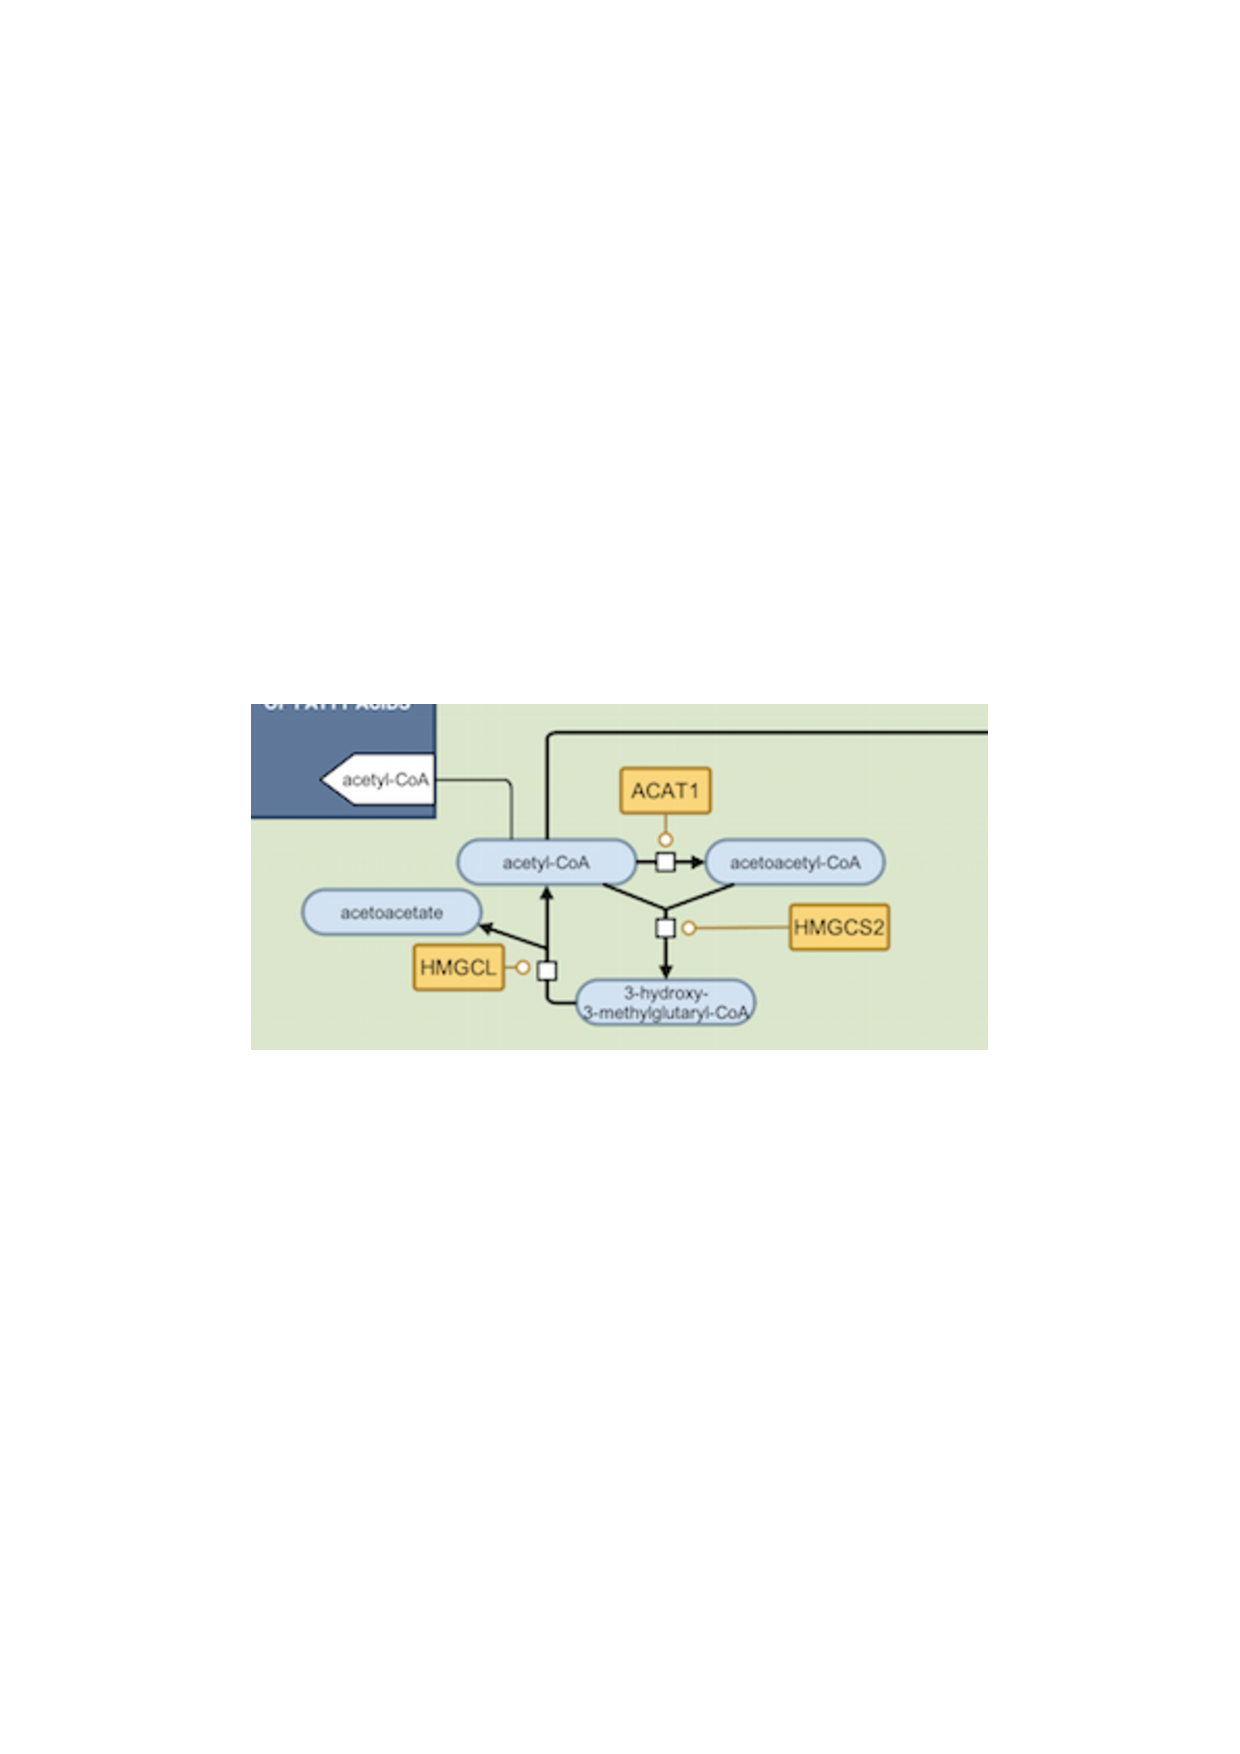
\includegraphics[width=\linewidth,clip,trim=5cm 12cm 5cm 12.5cm]{worked_example_ideas/example1_1}
\caption{An excerpt of Acetyl CoA metabolism drawn in SBGN. The
  correct interpretation is described in the text.}
\label{fig:weg1}
\end{figure}

 Generally in SBGN, the exact nature of a process is not shown by the
process node glyph, but is described by its interaction with other
glyphs. Thus we can see that process (4) in the example takes
acetyl-CoA and acetoacetyl-CoA as substrates and produces
3-hydroxy-3-methylglutaryl-CoA in a reaction catalysed by HMGCS2.


\section{Example 2: Cell Signalling}

In the previous example we describe reactions where one molecular
species is converted into another form. In this example
(figure~\ref{fig:weg2}) you can see how \PD describes cell signalling
processes. 

\begin{figure}[htb]
\includegraphics[width=\linewidth,clip,trim=5cm 12cm 5cm 12.5cm]{worked_example_ideas/cellsignalling_eg}
\caption{An excerpt of the Wnt signalling pathway in SBGN. The
  correct interpretation is described in the text.}
\label{fig:weg2}
\end{figure}


\section{Example 3: Transport}


\section{Example 4: Events and Phenotypes}

